\section{Results and Discussion}

\subsection{Performance Analysis}
This chapter supplies some benchmarks, to analyze how close this thesis came to achieving the wanted performance, which should be on eye level with C.

If not stated otherwise, benchmarks are written for this thesis and executed on an Intel Core i5-4200U with an HD 4400 graphic and 8GB of RAM.
Benchmarks were run on an idle computer with as little background processes running as possible.
The sources of the benchmarks can be found on Github.

\subsubsection{Julia}

Julia's performance is crucial for this thesis. 
If Julia doesn't perform close to C it would weaken the whole argument of writing the visualization library in Julia.
It is a very tedious task to write representative benchmarks for a language. The only way out is to rely on a multitude of sources and try to find analytical arguments.
In this thesis, Julia's own benchmark suite will be used in addition to some real world benchmarks from the Julia-Mailing list, where users ported code from some other language to Julia.
In addition, the general compiler structure of Julia will be analyzed to find indicators for Julia's overall performance.

\vspace{1em}
\begin{minipage}{\linewidth}
    \centering
    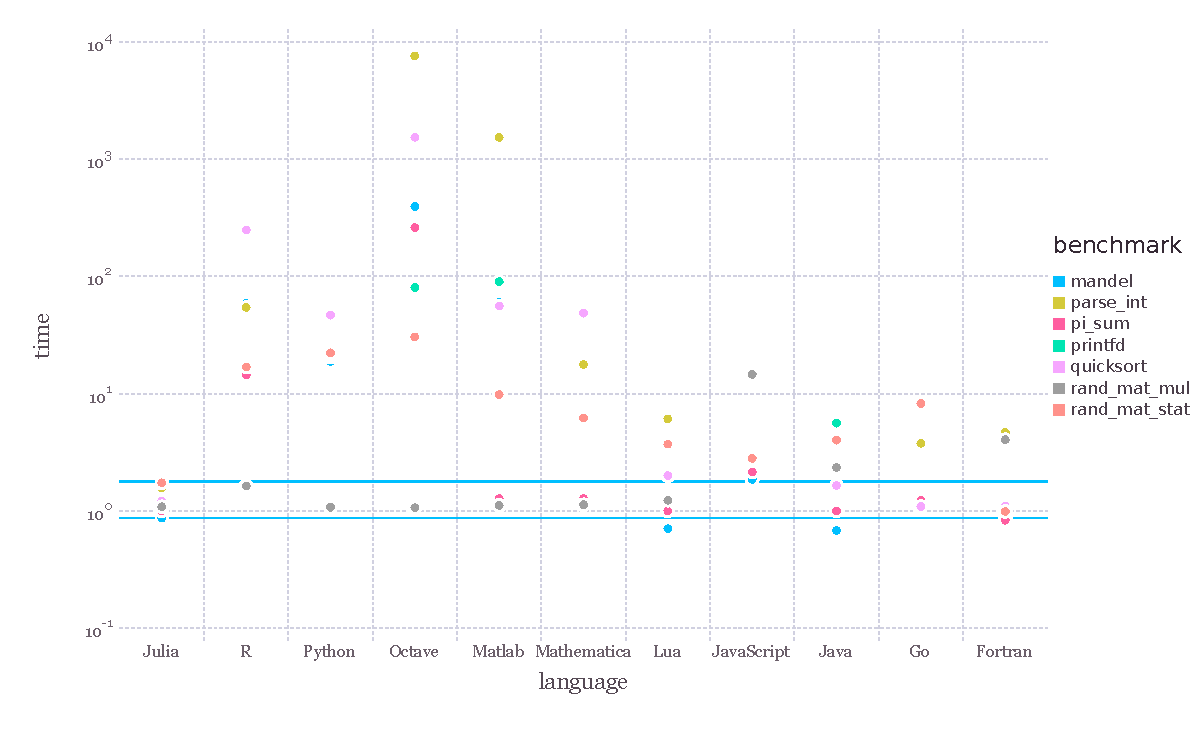
\includegraphics[width=0.9\linewidth]{graphics/juliabench.pdf}
    \captionof{figure}[Julia Performance]{Julia's performance compared to other languages, taken from Julia's micro bench suite \cite{JuliaBench}. Smaller is better, C performance = 1.0.}
    \label{fig:juliabench}
\end{minipage}

In the first benchmark from figure \ref{fig:juliabench}, we can see that Julia stays well within the range of C Speed. 
Actually, it even comes second to C-speed with no other language being that close.
This is a very promising first look at Julia, but it should be noted, that these benchmarks are written by the Julia core team.
So it is not guaranteed, that there is not a bias favoring Julia in these Benchmarks.
There is another benchmark comparing C++, Julia and F#, which was created by Palladium Consulting which should not have any interest in favoring one of the languages.
They compare in a blog post series \cite{JuliaFSCpp} the performance of C++, Julia and F# for an IBM/370 floating point to IEEE floating point conversion algorithm.
F# comes out last with 748.275 ms, than Julia with 483.769 ms and finally C++ with 463.474 ms. 
At the citation time, the Author had updated the C++ version to achieve 388.668 ms. 
This will be ignored, as it can not be said, if the other versions could not have been made faster with some more work as well.

The last benchmark is more real world oriented. 
It is Finite Element solver, which is an often used algorithm in material research and therefore represents a relevant use case for Julia.

\begin{table}[htbp]
    \centering
    \begin{tabular}{l|c|c|c}
        \hline
        \textbf{N}  & \textbf{Julia} & \textbf{FEniCS(Python + C++)}  & \textbf{FreeFem++(C++)}\\
        \hline
        121         & 0.99           & 0.67             & 0.01 \\
        2601        & 1.07           & 0.76             & 0.05 \\
        10201       & 1.37           & 1.00             & 0.23 \\
        40401       & 2.63           & 2.09             & 1.05 \\
        123201      & 6.29           & 5.88             & 4.03 \\
        251001      & 12.28          & 12.16            & 9.09 \\
        \hline
    \end{tabular}
    \captionof{table}[FEM Benchmark]{Performance of a FEM solver written in Julia compared to some existing libraries. \cite{FMSolver}}
    \label{table:fembench}
\end{table}
These are remarkable results, considering the small effort needed to program this in Julia, while being able to compete with established FEM solvers written in C++.


This list could go on an and, but it is more constructive, to find out Julia's limit and analyze the reasons for Julia being so fast.
As already mentioned, Julia is statically compiled at runtime. This means, as long as all types can be inferred, Julia will have in the most cases identical performance to C++.
The biggest remaining difference in this case is the garbage collector. I won't go much into detail here, as Julia's garbage collector is pretty young and only the future will show how big the actual difference will be. As seen in the benchmarks, it does not necessarily introduce big slowdowns. But there have been cases on the Julia mailing list, where large parts of code had to be changed in order to avoid that the garbage collector is the biggest bottle neck.

The other remaining difference to other technologies will then be, the difference in between different compiler technologies.
\ac{LLVM} biggest rival is \ac{gcc}. If C++ code compiled with \ac{gcc} is much faster than when it is compiled with \ac{LLVM}, Julia will also be much slower than the \ac{gcc} version.
In order to investigate this, one last benchmark will be analyzed.
This is the summary of the Phoronix benchmark suite run with \ac{gcc} and \ac{LLVM}:
\begin{table}[ht]
  \centering
  \begin{tabular}{l|c|c}
    \hline
    \textbf{Method} & \textbf{\ac{gcc} vs \ac{LLVM} 3.5} & \textbf{\ac{LLVM} 3.5 vs \ac{LLVM} 3.6} \\
    \hline
    mean & 0.99 & 0.99 \\
    median & 0.97 & 1.00 \\
    maximum & 1.48 & 1.10 \\
    minimum & 0.39 & 0.88 \\
    \hline
  \end{tabular}
    \captionof{table}[gcc vs llvm summary]{Summary of the Phoronix benchmark. Unit is speedup of LLVM, bigger is better. \cite{LLVM35vsLLVM36}\cite{LLVMvsGCC}\cite{Phoronix}}
    \label{table:gccvsllvm}
\end{table}

The full tables can be found in the appendix under the table \ref{table:llvm35vsllvm36} and \ref{table:llvmvsgcc}.
The results suggest, that \ac{LLVM} is well in the range of \ac{gcc}, even though that there can be big differences between the two.
This is quite comforting, especially if you consider, that LLVM is much younger than gcc. With Apple betting on LLVM, it is to be expected that \ac{LLVM} will stay competitive, which means Julia should in theory stay competitive as well.



\subsubsection{ModernGL}
\vspace{1em}
\begin{minipage}{\linewidth}
    \centering
    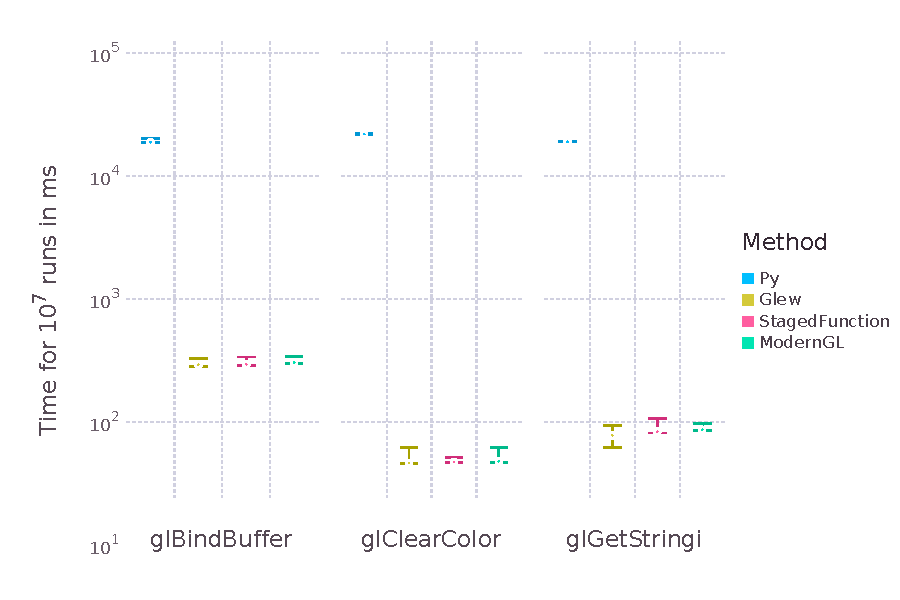
\includegraphics[width=0.9\linewidth]{graphics/glbench.pdf}
    \captionof{figure}[OpenGL Wrapper]{Different performance of OpenGL wrappers. The time for $10^7$ calls was measured 100 times for each function.}
    \label{fig:openglwrapper}
\end{minipage}
\begin{table}[htbp]
    \centering
    \begin{tabular}{l|c|c}
        \hline
        \textbf{Function}   & \textbf{Python}    & \textbf{Julia StagedFunction} \\
        \hline
        glBindBuffer        & 64.43              & 1.00\\
        glClearColor        & 474.72             & 1.02\\
        glStringi           & 244.44             & 1.07\\
    \end{tabular}
    \captionof{table}[OGL Relative Speed]{Performance relative to C++ with Glew (slowdown, bigger is worse)}
    \label{table:relativespeedoglw}
\end{table}

The OpenGL function loader from ModernGL has undergone some changes over the time. 
Starting with a very simple solution, there have been pull requests to include better methods for the functional loading.
The current approach wasn't written by me but by the Github user aaalexandrov.
I have experimented with a pretty new Julia feature, namely staged functions, for function loading which in principle should yield the best performance as it directly inlines the function pointer.
ModernGL gets benchmarked against Glew (with C++), PyOpenGL (with Python). From ModernGL itself, aaalexandrov's approach and the staged function approach are benchmarked.
These libraries where chosen by popularity, which was determined via Google search rank and development status and ranking on Github.
Like this, it should be guaranteed that they are the representative wrappers for the language.

The results can be seen in figure \ref{fig:openglwrapper}.
ModernGL seems to do pretty well compared to C++ and python does very badly, with being roughly 400 times slower for glClearColor.
Julia in contrast stays pretty much offers the same speed as C++ as can be seen in table \ref{table:relativespeedoglw}.
As all the OpenGL wrappers are pretty mature by now and bind to the same C library, this should mainly be a C function call benchmark.
Python does very bad here, but it must be noted that there are a lot of different Python distributions, where some of the promise to have better C interoperability. As this benchmarks goal is to show that Julia's ccall interface is comparable to a c function call from inside C++, the python options haven't been researched that thoroughly.
From this benchmark can be concluded, that Julia offers a solid basis for an \ac{OpenGL} wrapper library.

\subsubsection{Reactive}

\vspace{1em}
\begin{minipage}{\linewidth}
    \centering
    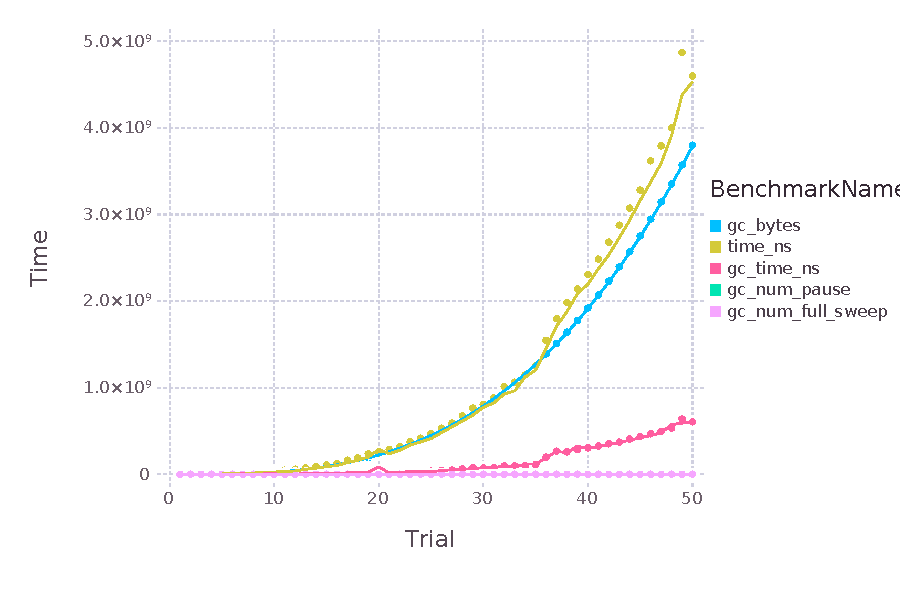
\includegraphics[width=0.9\linewidth]{graphics/react_bench.pdf}
    \captionof{figure}[Reactive 1]{Reactives performance for high memory, simple event graph}
    \label{fig:reactive1}
\end{minipage}
\vspace{1em}
\begin{minipage}{\linewidth}
    \centering
    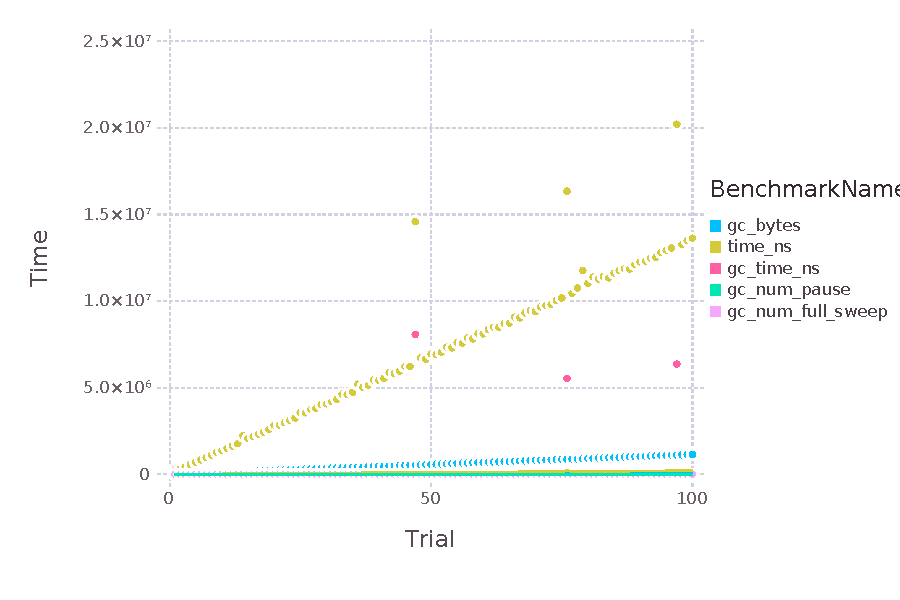
\includegraphics[width=0.9\linewidth]{graphics/react_bench2.pdf}
    \captionof{figure}[Reactive 2]{Reactives performance for complicated graph, simple calculation}
    \label{fig:reactive1}
\end{minipage}


\subsubsection{IJulia}
First of all, IJulia uses ZMQ to bridge the web interface with the Julia instance.
ZMQ is a messaging system using different sockets for communication like inproc, IPC, TCP, TIPC and multicas.
While it is very fast at it's task of sending messages, it can't compete with the native performance of staying inside one language.
This is not very important as long as there doesn't have to be much communication. This changes drastically for animations, where big memory chunks have to be streamed.



\subsection{Extensibility Analysis}

The modular design of Romeo has proven to be very effective and the goal of re-usability has already proven itself.
Most of the created modules are used independently by different people.
GLVisualize is used by myself for two packages, namely GLPlot, a scientific plotting package for Julia and for a prototype of a file explorer. 
It got forked by several users to create their own dynamic visualization packages.
The same applies for ModernGL and GLAbstraction. Most other used packages are at least used by one other project.
This indicates, that the abstraction and modularity is well designed, so that all the modules can function on their own.

The only exception is GLWindow, which has been used just indirectly through the other packages. 
This can mean three things.
First, it is badly abstracted and doesn't cleanly wrap one use case.
Secondly, it can be that the use case is not entirely clear to other people, which would not be a big surprise considering the minimal amount of documentation for GLWindow.
And finally, considering the small group of people developing graphics for Julia, it could be that they simply don't need the lower level functionality of GLWindow and instead rely on my other packages that use GLWindow.

Modularity guarantees a broad user and developer base, which in turn results in rich functionality and stability.
From further analyzing the Github repository written for this thesis, one can find out that there is a general lack of documentation.
This hinders people from contributing and using the packages.

The implementation in just one language has been achieved by choice. There are only a few exceptions, like the kernel code for OpenGL shaders, which can currently not be written in Julia. 
Julia programmers that use Romeo can extend Romeo with Julia and immediately see their results without complicated compilations.
This together with the speed is one of the main achievements compared to other libraries offering similar functionality, like IJulia, VTK and Matlab.
To further proof this point I will analyze the mentioned software in more detail.
The language usage statistics and necessary tools needed in order to extend the software will be the main focus of the analysis.
One needs to note, that the usage statistic of languages is just a weak indicator for the extendability of a software.
Using different languages for one project can make sense, if the project has different domains where domain specific languages give an advantage.
This chapter will only discuss the complexity introduced by languages, which are only needed for compatibility with other libraries or because the main language is too slow.

\subsubsection{IJulia}
Used languages:
IJUlia is written in Julia and relies on ZMQ(C++) and IPython. 
IPython uses multiple javascript rendering back-ends like Three.js and D3.
\begin{table}[htbp]
    \centering
    \begin{tabular}{l|l}
        \hline
        \textbf{Software} & \textbf{languages used}\\
        \hline
        IPython     & Python 78.5\% JavaScript:15.1\% HTML 5.0\% Other 1.4\%\\
        Three.js:   & JavaScript 62.4\% HTML 26.4\% Python 6.9\% C++ 1.9\% C 1.3\% GLSL 0.6\%\\
        D3:         & JavaScript 95.6\% CSS 4.3\%\\
        \hline
        \end{tabular}
    \captionof{table}[IJulia Stack]]{Technologies used in IJulia. Statistics taken from Github}
    \label{table:ijuliastack}
\end{table}
[more to come]
\subsubsection{Paraview and VTK}

Table \ref{table:ParaviewStatistic} in the appendix shows an extensive summary of the used languages in the Paraview repository.
It amounts to a total of 3.642.105 lines of code written in 29 languages.
[more to come]

\subsubsection{Matlab}

Matlab is closed source, which makes the core of Matlab impossible to extend.
This is why Matlab relays on a plug-in architecture, which enables developers to write closed or open source plug-ins for Matlab.
[Analysis of the plug-in Architecture]
[more to come]
\subsection{Usability Analysis}
[Consistency and ease of use of programming API in GLVisualize and Romeo.
Short comment about the \ac{GUI}]
